\section{Auswertung}
\label{sec:Auswertung}

Die Messwerte die wie in Abschnitt \ref{subsec:charak} beschrieben, aufgenommen wurden sind in Tabelle \ref{tab:imps} aufgelistet worden.
In der Abbildung \ref{fig:imps} wurden diese grafisch aufgetragen.
Die Grafik wurde mit dem python Plugin matplotlib \cite{matplotlib} erstellt.
Dabei ergibt sich der Fehler der Werte aus $\Delta N = \sqrt{N}$.
In der Grafik  ist ebenfalls eine Ausgleichsgerade zu sehen.
Diese wurde mit dem python Plugin scipy \cite{scipy} erstellt.
Die Werte mit denen die Ausgleichsgerade berechnet wurden, sind dabei die Werte die das Plateau bilden.
Zur Bestimmung der Qualität des Zählrohrs wurde nun die Steigung des Plateaus mithilfe der zuvor genannten Ausgleichsgeraden angenähert.
Dazu wurde diese nach dem Muster 
\begin{equation*}
  f(x) = ax +b 
\end{equation*} 
erstellt.
Die Wert der Steigung $a$ und der Wert $b$ sind dabei
\begin{align*}
  a =& \SI{1.16(22)}{\frac{\text{Imp}}{\A}} \\
  b =& \SI{9.58(11)e03}{\frac{\text{Imp}}{\second}}\\
\end{align*}
Die Fehler bei der Rechnung und allen folgenden wurden mit dem python Plugin \cite{uncertainties} berechnet.
Dieses nutzt die Gausschen-Fehlerfortpflanzungsformel 
\begin{equation*}
  \Delta y = \sqrt{\frac{\partial y}{\partial x_1}\Delta x_1+...}.
\end{equation*}

\begin{figure}
  \centering
  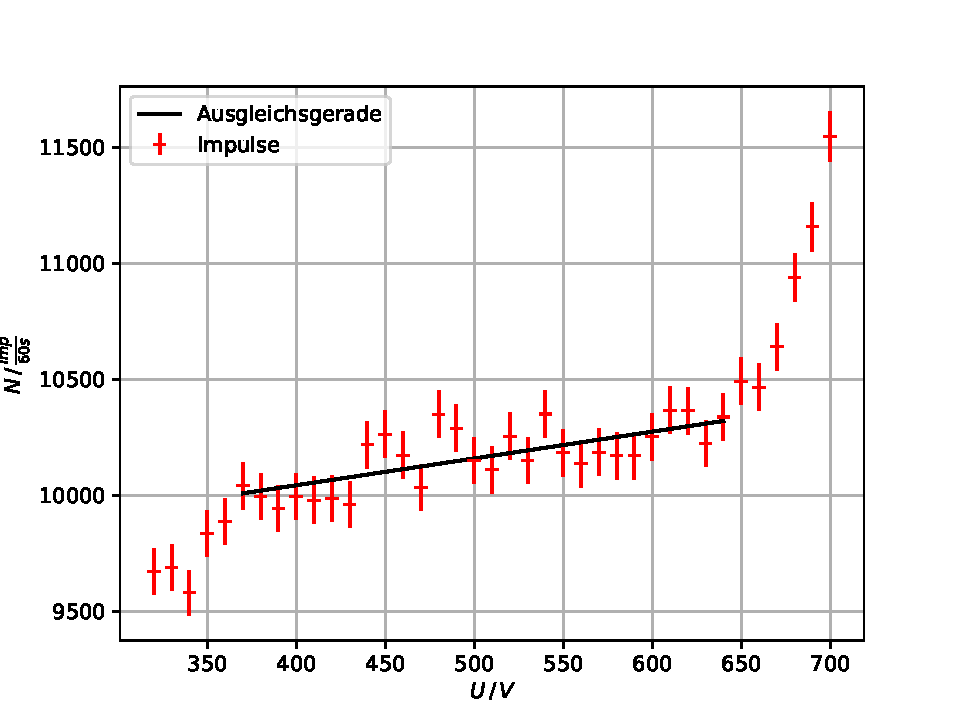
\includegraphics[width=0.6\textwidth]{content/data/kennlinie.pdf}
  \caption{Die aufgenommenen Messwerte mit zugehörigen Fehlern, sowie die Ausgleichsgerade.}
  \label{fig:imps}
\end{figure}

\begin{table}
  \centering
  \caption{Die gemessenen Impulse pro $60\si{\second}$ in Abhängigkeit von der Spannung des Zählrohrs.}
  \begin{tabular}[t]{cc}
    \toprule
    $U \, /\, \si{\V}$ & $N \,/\, \frac{\text{Imp}}{\si{\second}}$\\
    \midrule
    320 & 9672    \\
    330 & 9689    \\
    340 & 9580    \\
    350 & 9837    \\
    360 & 9886    \\
    370 & 10041   \\
    380 & 9996    \\
    390 & 9943    \\
    400 & 9995    \\
    410 & 9980    \\
    420 & 9986    \\
    430 & 9960    \\
    440 & 10219   \\
    450 & 10264   \\
    460 & 10174   \\
    470 & 10035   \\
    480 & 10350   \\
    490 & 10290   \\
    500 & 10151   \\
    510 & 10110   \\
    \bottomrule
  \end{tabular}
  \begin{tabular}[t]{cc}
    \toprule
    $U \, /\, \si{\V}$ & $N \,/\, \frac{\text{Imp}}{\si{\second}}$\\
    \midrule
    520 & 10255   \\
    530 & 10151   \\
    540 & 10351   \\
    550 & 10184   \\
    560 & 10137   \\
    570 & 10186   \\
    580 & 10171   \\
    590 & 10171   \\
    600 & 10253   \\
    610 & 10368   \\
    620 & 10365   \\
    630 & 10224   \\
    640 & 10338   \\
    650 & 10493   \\
    660 & 10467   \\
    670 & 10640   \\
    680 & 10939   \\
    690 & 11159   \\
    700 & 11547   \\
    \bottomrule
  \end{tabular}
\label{tab:imps}
\end{table}